\chapter{Análisis} 
\label{sec:analisis}

\section{Descripción detallada de la solución}

Se implementará una tienda de comercio electrónico utilizando Wordpress y su extensión WooCommerce. Por defecto, este plugin permite a los usuarios puntuar los productos por medio de un sistema de estrellas. A partir del código ya existente, se introducirán modificaciones para automatizar el proceso de valoración de los comentarios mediante IA.

Con este objetivo se construirá una aplicación software que utilice Cloud Natural Language, una herramienta de procesamiento del lenguaje natural, para evaluar los comentarios que se vayan publicando. El resultado obtenido se mostrará gráficamente junto a su respectivo comentario en la página web.

Se pretende también desarrollar una interfaz conversacional que actúe como un empleado del servicio de atención al cliente, permitiendo a los usuarios realizar consultas, solicitar recomendaciones o presentar quejas, entre otras acciones. 

Esta herramienta se integrará en la página web mediante un chat que será visible y accesible desde cualquier menú de la tienda. A partir de una petición, el chatbot intentará establecer una coincidencia con las respuestas que tiene programadas y proporcionará una contestación al cliente. El usuario podrá entablar una conversación con el bot sin preocuparse por el tipo de lenguaje empleado, y la interfaz deberá comprender la intención sin necesidad de que exista una coincidencia exacta con el registro de datos que posee.

No se persigue con este proyecto implementar un servicio muy amplio o robusto, sino presentar el potencial que tienen estas herramientas al ser aplicadas a una tienda electrónica.

\newpage

\section{Casos de uso del sistema}

En esta sección se detallan los casos de uso del sistema, incluyendo un diagrama de casos de uso, la especificación de los actores y la de cada uno de los casos de uso.

\subsection{Diagramas de casos de uso}


En el diagrama mostrado en la figura 4.1 se resumen visualmente aquellos casos de uso del sistema estrechamente ligados a la interacción del usuario con la aplicación de análisis de sentimientos y el bot conversacional.

\begin{figure}[ht]
	\begin{center}
		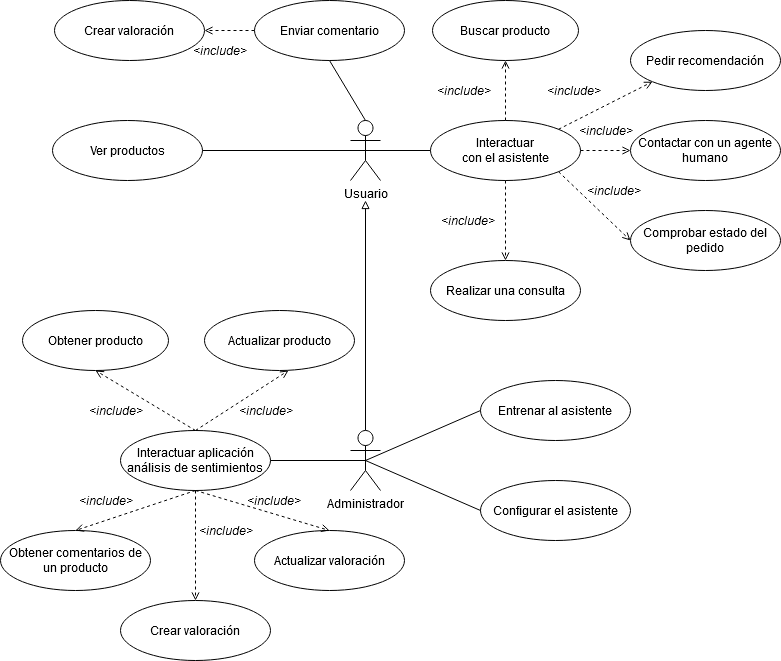
\includegraphics[width =\textwidth]{Figuras/DiagramaCasosUso.png}
	\end{center}
	\caption{\label{fig:casosUso} Diagrama de casos de uso}
\end{figure}

\newpage

\subsection{Descripción de actores del sistema}

A continuación, se describen los actores del sistema (A):

\begin{table}[htbp]
  \centering
    \scalebox{0.85}[0.85] {
    \begin{tabular}{l p{32.145em}}
    \toprule
    \textbf{A001} & \textbf{Usuario} \\
    \midrule
    Requisitos asociados & RF001, RF002, RF003, RF008, RF009, RF010, RF011, RF012, RF013. \\
    Descripción & Formado por todas las personas que accedan a la página web. \\
    Comentarios & Ninguno. \\
    \midrule
    \end{tabular}%
    }
  \label{tab:a003}
\end{table}%

\begin{table}[!htbp]
  \centering
  \scalebox{0.85}[0.85] {
    \begin{tabular}{l p{32.145em}}
    \toprule
    \textbf{A002} & \textbf{Administrador} \\
    \midrule
    Requisitos asociados & RF001, RF002, RF003, RF004, RF005, RF006, RF007, RF008, RF009, RF010, RF011, RF012, RF013, RF014, RF015. \\
    Descripción & Formado por las responsables del sistema. \\
    Comentarios & Ninguno. \\
    \midrule
    \end{tabular}%
  }
  \label{tab:a002}
\end{table}%

\subsection{Descripción de casos de uso del sistema}

Se procede a especificar los casos de uso del sistema que han sido identificados:

\begin{table}[htbp]
  \centering
  \scalebox{0.85}[0.85] {
    \begin{tabular}{l p{32.145em}}
    \toprule
    \textbf{RF0001} & \textbf{Ver productos} \\
    \midrule
    Requisitos asociados & Ninguno. \\
    Descripción & Un usuario (A001) podrá acceder al catálogo completo de productos disponibles en la tienda. \\
    Precondición & Ninguna. \\
    Postcondición & Ninguna.\\
    Comentarios & Ninguno. \\
    \midrule
    \end{tabular}%
  }
  \label{tab:rf001}
\end{table}%

\begin{table}[!htbp]
  \centering
    \scalebox{0.85}[0.85] {
    \begin{tabular}{l p{32.145em}}
    \toprule
    \textbf{RF0002} & \textbf{Enviar comentario} \\
    \midrule
    Requisitos asociados & RNF002. \\
    Descripción & Un usuario (A001) podrá publicar su opinión sobre un producto. \\
    Precondición & Ninguna. \\
    Postcondición & El sistema mostrará el comentario introducido.\\
    Comentarios & Si el usuario no ha iniciado sesión, el comentario será publicado como anónimo. \\
    \midrule
    \end{tabular}%
  }
  \label{tab:rf002}
\end{table}%

\begin{table}[htbp]
  \centering
  \scalebox{0.85}[0.85] {
    \begin{tabular}{l p{32.145em}}
    \toprule
    \textbf{RF0003} & \textbf{Crear valoración} \\
    \midrule
    Requisitos asociados & RNF002, RNF003, RNF004. \\
    Descripción & De forma general, sólo se creará una valoración cuando un usuario (A001) introduzca un comentario. Aunque el administrador (A002) podrá realizar una petición directa al servicio de la API. \\
    Precondición & Enviar un comentario o realizar una llamada a la API incluyendo un token de autenticación. \\
    Postcondición & Se actualizará el valor de puntuación y magnitud del comentario. \\
    Comentarios & La puntuación se muestra gráficamente en la tienda junto a la opinión evaluada. \\
    \midrule
    \end{tabular}%
  }
  \label{tab:rf003}
\end{table}%

\begin{table}[htbp]
  \centering
  \scalebox{0.85}[0.85] {
    \begin{tabular}{l p{32.145em}}
    \toprule
    \textbf{RF004} & \textbf{Obtener producto} \\
    \midrule
    Requisitos asociados & RNF004. \\
    Descripción & Un administador (A002) solicita información sobre un producto. \\
    Precondición & Incluir un token de autenticación y un nombre de producto válidos. \\
    Postcondición & Se ofrecerá el nombre, ID y puntuación media del producto. \\
    Comentarios & La puntuación es la media de los comentarios del producto. \\
    \midrule
    \end{tabular}%
  }
  \label{tab:rf004}
\end{table}%

\begin{table}[htbp]
  \centering
  \scalebox{0.85}[0.85] {
    \begin{tabular}{l p{32.145em}}
    \toprule
    \textbf{RF005} & \textbf{Actualizar producto} \\
    \midrule
    Requisitos asociados & RNF004. \\
    Descripción & Un administador (A002) solicita actualizar la puntuación de un producto. \\
    Precondición & Incluir un token de autenticación y un nombre de producto válidos. \\
    Postcondición & Se ofrecerá el nombre, ID y puntuación media del producto. \\
    Comentarios & La puntuación es la media de los comentarios del producto. \\
    \midrule
    \end{tabular}%
  }
  \label{tab:rf005}
\end{table}%


\begin{table}[htbp]
  \centering
  \scalebox{0.85}[0.85] {
    \begin{tabular}{l p{32.145em}}
    \toprule
    \textbf{RF006} & \textbf{Obtener comentarios de un producto} \\
    \midrule
    Requisitos asociados & RNF004. \\
    Descripción & Un administador (A002) solicita los comentarios de un producto. \\
    Precondición & Incluir un token de autenticación y un ID de producto válidos. \\
    Postcondición & Se listarán todos los comentarios pertenecientes a dicho producto. \\
    Comentarios & Ninguno. \\
    \midrule
    \end{tabular}%
  }
  \label{tab:rf006}
\end{table}%

\newpage

\begin{table}[htbp]
  \centering
  \scalebox{0.85}[0.85] {
    \begin{tabular}{l p{32.145em}}
    \toprule
    \textbf{RF007} & \textbf{Actualizar valoración} \\
    \midrule
    Requisitos asociados & RNF002, RNF003, RNF004. \\
    Descripción & Un administador (A002) solicita actualizar la valoración de un comentario. \\
    Precondición & Incluir un token de autenticación y un ID de comentario válidos. \\
    Postcondición & Se ofrecerá el ID, autor, contenido, puntuación y magnitud del comentario. \\
    Comentarios & Ninguno. \\
    \midrule
    \end{tabular}%
 }
  \label{tab:rf007}
\end{table}%

\begin{table}[!htbp]
  \centering
  \scalebox{0.85}[0.85] {
    \begin{tabular}{l p{32.145em}}
    \toprule
    \textbf{RF008} & \textbf{Interactuar con el chatbot} \\
    \midrule
    Requisitos asociados & RNF001. \\
    Descripción & Un usuario (A001) podrá entablar una conversación con el chatbot. \\
    Precondición & Ninguna. \\
    Postcondición & El agente presentará mediante un menú las acciones que puede realizar.\\
    Comentarios & Será accesible desde cualquier parte de la página web. \\
    \midrule
    \end{tabular}%
 }
  \label{tab:rf008}
\end{table}%

\begin{table}[htbp]
  \centering
  \scalebox{0.85}[0.85] {
    \begin{tabular}{l p{32.145em}}
    \toprule
    \textbf{RF009} & \textbf{Buscar producto} \\
    \midrule
    Requisitos asociados & RNF001. \\
    Descripción & Un usuario (A001) podrá solicitar la ayuda del chatbot para buscar un producto. \\
    Precondición & Seleccionar esta acción. \\
    Postcondición & El asistente preguntará al usuario acerca de la categoría y la marca del producto, ofreciendo un enlace a una selección de productos en función de las decisiones del usuario \\
    Comentarios & Ninguno. \\
    \midrule
    \end{tabular}%
  }
  \label{tab:rf009}
\end{table}%

\begin{table}[!htbp]
  \centering
  \scalebox{0.85}[0.85] {
    \begin{tabular}{l p{32.145em}}
    \toprule
    \textbf{RF010} & \textbf{Pedir recomendación} \\
    \midrule
    Requisitos asociados & RNF001. \\
    Descripción & Un usuario (A001) podrá solicitar una recomendación al chatbot.  \\
    Precondición &  Seleccionar esta acción.\\
    Postcondición & El asistente preguntará al usuario acerca de la categoría y la marca del producto, ofreciendo un enlace a una selección de productos en función de las decisiones del usuario. \\
    Comentarios & El chatbot recomendará el producto mejor valorado. \\
    \midrule
    \end{tabular}%
  }
  \label{tab:rf010}
\end{table}%

\begin{table}[htbp]
  \centering
  \scalebox{0.85}[0.85] {
    \begin{tabular}{l p{32.145em}}
    \toprule
    \textbf{RF011} & \textbf{Contactar con un agente humano} \\
    \midrule
    Requisitos asociados & RNF001. \\
    Descripción & Un usuario (A001) podrá solicitar contactar con un agente humano. \\
    Precondición & Seleccionar esta acción. \\
    Postcondición & El chatbot ofrecerá un enlace al formulario de contacto. \\
    Comentarios & Ninguno. \\
    \midrule
    \end{tabular}%
  }
  \label{tab:rf011}
\end{table}%

\begin{table}[htbp]
  \centering
  \scalebox{0.85}[0.85] {
    \begin{tabular}{l p{32.145em}}
    \toprule
    \textbf{RF012} & \textbf{Comprobar estado del pedido} \\
    \midrule
    Requisitos asociados & RNF001. \\
    Descripción & Un usuario (A001) podrá solicitar información sobre el estado de su pedido. \\
    Precondición & Seleccionar esta acción e introducir un número de pedido válido. \\
    Postcondición & El chatbot informará al usuario que recibirá un correo con la información de dicho pedido. \\
    Comentarios & Un número de pedido válido se compone de 5 cifras. \\
    \midrule
    \end{tabular}%
  }
  \label{tab:rf012}
\end{table}%

\begin{table}[htbp]
  \centering
  \scalebox{0.85}[0.85] {
    \begin{tabular}{l p{32.145em}}
    \toprule
    \textbf{RF013} & \textbf{Realizar una consulta} \\
    \midrule
    Requisitos asociados & RNF001. \\
    Descripción & Un usuario (A001) podrá plantear preguntas sobre su cuenta, pedido, formas de pago, envios, etc. \\
    Precondición & Seleccionar esta acción y formular la pregunta. \\
    Postcondición & El chatbot responderá de manera breve y adjuntará un enlace al centro de atención al cliente. \\
    Comentarios & Ninguno. \\
    \midrule
    \end{tabular}%
  }
  \label{tab:rf013}
\end{table}%

\begin{table}[htbp]
  \centering
  \scalebox{0.85}[0.85] {
    \begin{tabular}{l p{32.145em}}
    \toprule
    \textbf{RF014} & \textbf{Entrenar el asistente} \\
    \midrule
    Requisitos asociados & RNF001. \\
    Descripción &  El administrador (A002) puede añadir nuevos registros para aumentar el conocimiento del chatbot\\
    Precondición & Acceder al servicio de Dialogflow. \\
    Postcondición & Ninguna. \\
    Comentarios & Ninguno. \\
    \midrule
    \end{tabular}%
  }
  \label{tab:rf014}
\end{table}%


\begin{table}[htbp]
  \centering
  \scalebox{0.85}[0.85] {
    \begin{tabular}{l p{32.145em}}
    \toprule
    \textbf{RF015} & \textbf{Configurar el asistente} \\
    \midrule
    Requisitos asociados & RNF001. \\
    Descripción & El administrador (A002) pude modificar las funcionalidades del chatbot. \\
    Precondición & Acceder al servicio de Dialogflow. \\
    Postcondición & Ninguno. \\
    Comentarios & Ninguna. \\
    \midrule
    \end{tabular}%
  }
  \label{tab:rf015}
\end{table}%

\newpage
\section{Requisitos funcionales}

Los requisitos funcionales del sistema coinciden con los casos de uso expuestos en la sección anterior. Son los siguientes:

\begin{itemize}
    \item \textbf{RF001} Ver productos
    \item \textbf{RF002} Enviar comentario
    \item \textbf{RF003} Crear valoración
    \item \textbf{RF004} Obtener producto
    \item \textbf{RF005} Actualizar producto
    \item \textbf{RF006} Obtener comentarios de un producto
    \item \textbf{RF007} Actualizar valoración
    \item \textbf{RF008} Interactuar con el chatbot
    \item \textbf{RF009} Buscar producto
    \item \textbf{RF010} Pedir recomendación
    \item \textbf{RF011} Contactar con un agente humano
    \item \textbf{RF012} Comprobar estado del pedido
    \item \textbf{RF013} Realizar una consulta
    \item \textbf{RF014} Entrenar al asistente
    \item \textbf{RF015} Configurar el asistente
    
\end{itemize}

\section{Requisitos no funcionales}

Por un lado los requisitos no funcionales relacionados con la disponibilidad temporal del sitio web están fijados por los SLAs (Service Level Agreement) que establecen los servicios de Google Cloud y son:
\begin{itemize}
    \item El servicio Cloud Run debe estar disponible el 99.95\% del tiempo.
    \item La base de datos en Cloud SQL debe estar disponible el 99.95\% del tiempo.
    \item El servicio de Dialogflow debe permanecer activo más del 99.9\% del tiempo.
    \item El servicio de Natural Language debe estar también disponible más del 99.9\% del tiempo.
\end{itemize}

\newpage

El resto de requisitos no funcionales son:

\begin{table}[htbp]
  \centering
  \scalebox{0.85}[0.85] {
    \begin{tabular}{l p{32.145em}}
    \toprule
    \textbf{RNF001} & \textbf{Lenguaje soportado por el chatbot} \\
    \midrule
    Descripción & El lenguaje principal del bot conversacional será el español. \\
    Comentarios & Puede configurarse para soportar otros lenguajes. \\
    \midrule
    \end{tabular}%
  }
  \label{tab:rnf001}
\end{table}%

\begin{table}[htbp]
  \centering
  \scalebox{0.85}[0.85] {
    \begin{tabular}{l p{32.145em}}
    \toprule
    \textbf{RNF002} & \textbf{Lenguajes utilizados en los comentarios} \\
    \midrule
    Descripción & Los comentarios publicados por los clientes pueden ser en inglés, español, francés, alemán, italiano, japonés, coreano, portugués (brasileño y continental) y chino (simplificado y tradicional). \\
    Comentarios & Son los lenguajes soportados por Google NLP. \\
    \midrule
    \end{tabular}%
  }
  \label{tab:rnf002}
\end{table}%

\begin{table}[!htbp]
  \centering
  \scalebox{0.85}[0.85] {
    \begin{tabular}{l p{32.145em}}
    \toprule
    \textbf{RNF003} & \textbf{Sistema de puntuación} \\
    \midrule
    Descripción & La puntuación de los comentarios se mostrará en forma de estrellas. \\
    Comentarios & Ninguna. \\
    \midrule
    \end{tabular}%
  }
  \label{tab:rnf003}
\end{table}%

\begin{table}[!htbp]
  \centering
  \scalebox{0.85}[0.85] {
    \begin{tabular}{l p{32.145em}}
    \toprule
    \textbf{RNF004} & \textbf{Seguimiento de errores} \\
    \midrule
    Descripción & La aplicación de análisis de sentimientos deberá almacenar logs de los errores. \\
    Comentarios & El almacenamiento se realizará en la nube utilizando Cloud Logging. \\
    \midrule
    \end{tabular}%
  }
  \label{tab:rnf004}
\end{table}%

\section{Análisis económico}

\subsection{Tarifas de los servicios de Google Cloud}

\subsubsection{Google Natural Language Processing}

El precio de este servicio se calcula mensualmente según la funcionalidad utilizada y el número de unidades evaluadas. Cada petición realizada a la API supone una unidad; si contiene más de 1000 caracteres se cuenta una unidad por cada 1000 caracteres. Por ejemplo, si se envían tres peticiones que contienen 300, 1725 y 850 caracteres respectivamente, se llevará a cabo el cobro por 4 unidades.

A continuación, se muestran en una tabla los precios establecidos por Google por cada 1000 unidades según el total de unidades evaluadas a lo largo de un mes:

\begin{table} [htbp]
	\centering
    \scalebox{0.75}[0.75] {
	\begin{tabular}{l c c c c}
		\textbf{Función} & \textbf{0-5000} & \textbf{5001-1.000.000} & \textbf{1.000.001-5.000.000} & \textbf{5.000.000-20.000.000} \\ \hline
         Análisis de entidades & Gratis & 1 USD & 0,50 USD & 0,25 USD \\
         Análisis de opinión & Gratis & 1 USD & 0,50 USD & 0,25 USD \\
         Análisis sintáctico & Gratis & 0,50 USD & 0,25 USD & 0,125 USD \\
         Análisis de opinión de entidades & Gratis & 2 USD & 1 USD & 0,50 USD \\
	\end{tabular}}
	\centering
	\caption{\label{tab:costeNLP}Precios mensuales Cloud Natural Language. Fuente: Google Cloud.}
\end{table}

\newpage

\subsubsection{Cloud Run}

Dada una instancia de un contenedor, el tiempo de facturación comienza cuando la instancia está procesando al menos una petición. Si dicha instancia recibe varias peticiones al mismo tiempo, la facturación comienza cuando llega la primera petición y termina cuando se resuelve la última petición. En el siguiente diagrama se puede observar esta situación:

\begin{figure}[ht]
	\begin{center}
		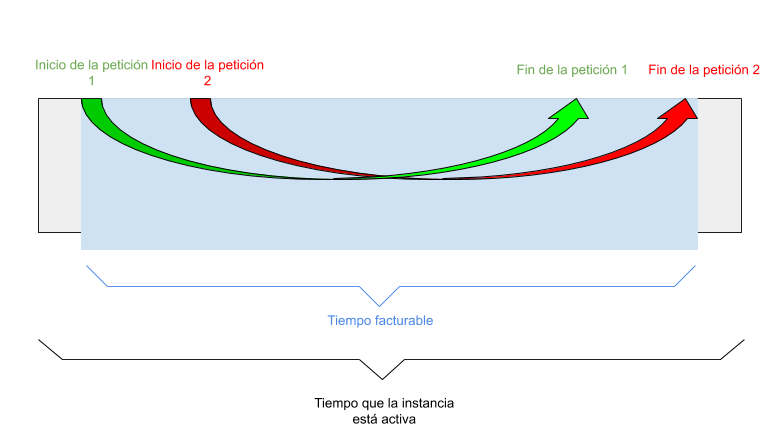
\includegraphics[width = 0.95\textwidth]{Figuras/FacturacionCloudRun.png}
	\end{center}
	\caption{\label{fig:facturacionCloudRun} Tiempo facturable Cloud Run. Fuente: Google Cloud.}
\end{figure}


A continuación, se exponen en una tabla los precios establecidos para el servicio utilizando como unidad el GiB/s, es decir ejecutar una instancia de 1 GiB durante un segundo. La unidad vCPU indica lo mismo, uso por segundo de vCPU.

\begin{table} [htbp]
	\centering
	 \scalebox{0.75}[0.75] {
	\begin{tabular}{l l l l}
		\textbf{CPU} & \textbf{Memoria} & \textbf{Solicitudes} & \textbf{Redes} \\ 
		\hline
		180.000 vCPU/s gratuitas &
		360.000 GiB gratuitos &
		2 millones gratuitas &
		1 GiB gratuito en Norteamérica \\
		
		0.000024 USD por vCPU/s &
		0.00000250 USD GiB/s &
		0,40 USD por millón &
		Depende de la geolocalización \\

	\end{tabular}}
	\centering
	\caption{\label{tab:costeCloudRun}Precios por uso de Cloud Run. Fuente: Google Cloud.}
\end{table}

Sólo se cobrará por el uso de Cloud Run cuando se supere la cantidad gratuita. Esta cuota es compartida por todos los proyectos pertenecientes a la misma cuenta de facturación y se renueva mensualmente.

\subsubsection{Cloud SQL}

El coste de este servicio depende principalmente del tipo de instancia utilizada y la región en la que se sitúe. Este cargo se calcula por minuto de ejecución de la instancia. Por ejemplo, el coste por mes de una instancia \textit{db-n1-standard-2} sería:

\begin{table} [htbp]
	\centering
	\scalebox{0.85}[0.85] {
	\begin{tabular}{c c c c c c c}
		\textbf{CPU} & \textbf{RAM} & \textbf{Almacenamiento} & \textbf{Conexiones} & 
		\textbf{Precio} & \textbf{Precio de alta disponibilidad}	\\ 
		\hline
         2 & 7,5 & 30.720 GB & 4000 & 49,31 USD & 98,62 USD\\
	\end{tabular}}
	\centering
	\caption{\label{tab:costeMySQL}Precios mensuales de instancias MySQL. Fuente: Google Cloud.}
\end{table}

Otras opciones de configuración como la capacidad de almacenamiento, el tipo (SSD o HDD) y el número de copias de seguridad también influyen en el precio final:

\begin{itemize}
    \item SSD: 0,170 USD por GB/Mes
    \item HDD: 0,090 USD por GB/Mes
    \item Copias de seguridad: 0,080 USD por GB/Mes
\end{itemize}

Además, pueden cobrarse cargos adicionales según el destino del tráfico a la salida de Cloud SQL: 

\begin{itemize}
    \item Instancias de Compute Engine y réplicas interregionales de Cloud SQL: si es en la misma región, gratis; 0,12 USD/GB entre regiones dentro y fuera de Norteamérica.
    \item Productos de Google (sin contar Compute Engine): si es intracontinental, gratis. En caso contrario 0,12 USD/GB.
    \item Salida a Internet a través de Cloud Interconnect: 0,05 USD/GB.
    \item Salida a Internet sin Cloud Interconnect: 0,19 USD/GB.
\end{itemize}

Por último, aspectos como el tiempo que el usuario se comprometa a hacer uso de este servicio también tienen impacto sobre el coste total. 

Con tantos factores influyendo sobre el coste total se puede comprobar que es difícil conocer exactamente la cuantía que deberá afrontar la empresa.

\subsubsection{Container Registry}

Para almacenar las imágenes en Container Registry se crea un segmento de almacenamiento de Cloud Storage, que de forma predeterminada es de tipo Standard. El coste para este tipo de segmentos es de 0,026 USD por GB al mes. 

\newpage

En la siguiente tabla aparecen reflejados los precios por GB al mes para cada tipo de segmento de Cloud Storage:

\begin{table} [htbp]
	\centering
	\begin{tabular}{l c c c c}
		\textbf{Standard} & \textbf{Nearline} & \textbf{Coldline} & \textbf{Archive} \\ \hline
         0.026 USD & 0.010 USD & 1 0.007 USD & 0.004 USD \\
	\end{tabular}
	\centering
	\caption{\label{tab:costeCloudStorage}Precios mensuales Cloud Storage. Fuente: Google Cloud.}
\end{table}

Si se desea realizar un análisis de vulnerabilidades sobre las imágenes subidas, supone un coste de 0,26 USD por imagen. Sin embargo, sólo se cobrará la primera vez que se analice cada imagen, es decir, no se cobran análisis posteriores sobre la misma imagen.

\subsubsection{Cloud Logging}

Los primeros 50 GiB usados por proyecto serán gratuitos, a partir de aquí se aplicará una tarifa de 0,50 USD por cada GiB adicional.

\subsubsection{Dialogflow}

Actualmente DialogFlow cuenta con tres planes diferentes de pago, como en este proyecto solo se hace uso de peticiones en forma de texto, se van a comparar estos planes en función de sus cuotas para texto.
\begin{itemize}
    \item \textbf{Edición estándar}. Es gratuito, pero se encuentra limitado por límite de peticiones que se pueden realizar; permite hasta un máximo de 180 solicitudes por minuto.
    \item \textbf{Edición empresarial}. Ofrece cuotas de uso más elevadas y además asistencia técnica por parte de Google Cloud. Dentro de esta edición se distinguen dos formatos:
    \begin{itemize}
        \item Essentials. Permite hasta 600 peticiones por minuto con un precio de 0,002 USD por solicitud.
        \item Plus. Se trata de la versión más avanzada, contiene todas las funcionalidades de Essentials y ofrece más opciones respecto a los conectores de conocimiento. Permite hasta 600 peticiones por minuto con un precio de 0,004 USD por solicitud.
    \end{itemize}
\end{itemize}


\subsection{Presupuesto de realización del proyecto}

Se procede a detallar el coste económico que ha supuesto la realización de este proyecto, para ello se tomará como referencia la estimación de horas expuesta en el apartado Fases de desarrollo. Conviene indicar que no sólo se tiene en cuenta el tiempo dedicado, también se consideran los costes asociados a los recursos utilizados durante el desarrollo.

\subsubsection{Costes directos}

Se entiende por costes directos aquellos que están directamente relacionados con el desarrollo del producto y la determinación el precio de venta. A continuación se exponen los costes directos a los que se ha tenido que hacer frente:

\begin{itemize}
    \item \textbf{Capital Humano}. Habría que establecer dos precios distintos para cada miembro debido a las diferencias de experiencia y conocimientos entre el autor y el alumno. Sin embargo, sólo se tendrá como referencia el trabajo realizado por el alumno para el cómputo del coste. Estableciendo un precio de 18€/hora, el coste total sería de:
    \begin{equation}
        300h \times 18\textup{€}/h = 5400\textup{€}
    \end{equation}
    \item \textbf{Hardware}. El único equipamiento hardware que se ha necesitado para el desarrollo del proyecto ha sido el de un ordenador portátil. En concreto, se trata de un ordenador MSI con 8 GB de memoria RAM y un procesador i7. En el momento de su adquisición supuso un coste de 800€.
    \item \textbf{Software}. Todo el software utilizado es gratuito, sin embargo cabe destacar que los servicios cloud utilizados no han supuesto ningún coste adicional porque se han utilizado sus planes más básicos que suelen ser gratuitos. Una vez que el sistema se encuentre en funcionamiento, quizás el plan más básico no sea suficiente y haya que aumentar las prestaciones ocasionando un incremento de los gastos.
\end{itemize}

\subsubsection{Costes totales}

Para obtener el coste total del proyecto, se añaden a los costes directos un 20\% de los mismos en concepto de costes indirectos.

\begin{table} [htbp]
	\centering
	\begin{tabular}{l c c}
		\textbf{Tipo de coste} & \textbf{Importe}\\ \hline
         Capital humano & 5400€ \\
         Hardware & 800€ \\
         Software & 0€ \\
         Costes indirectos & 1240€ \\
         \hline
         Coste total & 7440€ \\ 
	\end{tabular}
	\centering
	\caption{\label{tab:presupuesto}Presupuesto}
\end{table}

Los costes indirectos reflejados en el cálculo del presupuesto son aquellos en los que incurre la empresa pero que no puede imputar directamente al proceso de producción. Aquí se incluyen los gastos ocasionados por la factura de luz e internet, el desplazamiento para acudir a tutorías con el tutor, etc.